\documentclass[12pt]{article}

% Opening
\title{Applied Combinatorics Homework 3}
\author{Akash Narayanan}
\usepackage{amsmath, amsfonts, amssymb, amsthm, enumitem, tikz}
\usepackage{caption, subcaption, float}

% Problem counters
\newcounter{chapternumber}


% Problem environment
\theoremstyle{definition}
\newtheorem{problem-internal}{Problem}[chapternumber]
\newenvironment{problem}{
  \medskip
  \begin{problem-internal}
}{
\end{problem-internal}
}

% Solution environment
\newenvironment{solution}{
  \begin{proof}[Solution]
    \vspace{-8px}
    \setlength{\parskip}{4px}
    \setlength{\parindent}{0px}
}{
\end{proof}
}

\newtheorem*{proposition}{Proposition}

\begin{document}

  \maketitle

  % Problem 5.21
  \setcounter{chapternumber}{5}
  \setcounter{problem-internal}{20}
  \begin{problem}
    Find a recursive formula for the number of vertices \(n_{t}\) in the graph \textbf{G}\textsubscript{\(t\)} from the proof of the below proposition.
  \end{problem}

  \begin{proposition}
    For every \(t \geq 3\), there exists a graph \textbf{G}\textsubscript{\(t\)} so that \(\chi \left( \text{\textbf{G}\textsubscript{\(t\)}} \right) = t\) and \(\omega \left( \text{\textbf{G}\textsubscript{\(t\)}} \right)\) = 2.
  \end{proposition}

  \begin{solution}
    \textbf{G}\textsubscript{3} is defined as \textbf{C}\textsubscript{5} so \(n_{3} = 5\). In general, if \textbf{G}\textsubscript{\(t\)} has \(n_{t}\) vertices, we form \textbf{G}\textsubscript{\(t+1\)} as follows. We begin with an independent set \(I\) which has \(n_{t}\) points labelled \(y_{1}, y_{2}, \ldots, y_{n_{t}}\). Then we add a copy of \textbf{G}\textsubscript{\(t\)} with \(y_{i}\) adjacent to \(x_{j}\) if and only if \(x_{i}\) is adjacent to \(x_{j}\). At this point, we have added another \(n_{t}\) vertices to our graph. Finally, a new vertex \(z\) is adjacent to all vertices in \(I\). Therefore, we have the following recursive formula:
    \begin{align*}
      n_{t+1} = 2n_{t} + 1
    \end{align*}
  \end{solution}

  % Problem 5.39
  \setcounter{problem-internal}{38}
  \begin{problem}
    Determine pr\"{u}fer(\textbf{T}) for the tree \textbf{T} shown below.

    \begin{figure}[H]
      \centering
      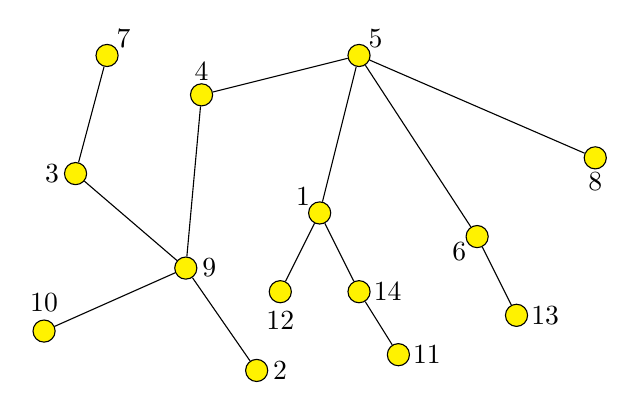
\begin{tikzpicture}
        [scale=1,every node/.style={draw,shape=circle,fill=yellow,inner sep=0,minimum size=8pt}, every draw/.style={line width=0.25mm, black}]

        \node[label=135:{1}] (v1) at (0, 0) {};
        \node[label=0:{2}] (v2) at (-0.8, -2) {};
        \node[label=180:{3}] (v3) at (-3.1, 0.5) {};
        \node[label=90:{4}] (v4) at (-1.5, 1.5) {};
        \node[label=45:{5}] (v5) at (0.5, 2) {};
        \node[label=215:{6}] (v6) at (2, -0.3) {};
        \node[label=45:{7}] (v7) at (-2.7, 2) {};
        \node[label=270:{8}] (v8) at (3.5, 0.7) {};
        \node[label=0:{9}] (v9) at (-1.7, -0.7) {};
        \node[label=90:{10}] (v10) at (-3.5, -1.5) {};
        \node[label=0:{11}] (v11) at (1, -1.8) {};
        \node[label=270:{12}] (v12) at (-0.5, -1) {};
        \node[label=0:{13}] (v13) at (2.5, -1.3) {};
        \node[label=0:{14}] (v14) at (0.5, -1) {};

        \draw (v1) -- (v5);
        \draw (v1) -- (v12);
        \draw (v1) -- (v14);
        \draw (v2) -- (v9);
        \draw (v3) -- (v7);
        \draw (v3) -- (v9);
        \draw (v4) -- (v5);
        \draw (v4) -- (v9);
        \draw (v5) -- (v6);
        \draw (v5) -- (v8);
        \draw (v6) -- (v13);
        \draw (v9) -- (v10);
        \draw (v11) -- (v14);

      \end{tikzpicture}
    \end{figure}
  \end{problem}

  \begin{solution}
    The table below shows the process.
    \begin{center}
      \begin{tabular}{c c}
        Unique Neighbor & Vertex Removed \\
        9  & 2  \\
        3  & 7  \\
        9  & 3  \\
        5  & 8  \\
        9  & 10 \\
        4  & 9  \\
        5  & 4  \\
        14 & 11 \\
        1  & 12 \\
        6  & 13 \\
        5  & 6  \\
        1  & 14
      \end{tabular}
    \end{center}
    Then pr\"ufer(\textbf{T}) is the string 9 3 9 5 9 4 5 14 1 6 5 1. Using spaces as delimiters helps distinguish between 1 4 and 14.
  \end{solution}

  % Problem 6.1
  \setcounter{chapternumber}{6}
  \setcounter{problem-internal}{0}
  \begin{problem}
    We say that a relation \(R\) on a set \(X\) is \textbf{\textit{symmetric}} if \(\left( x, y \right) \in R\) implies \(\left( y, x \right) \in R\) for all \(x, y \in X\). If \(X = \{a, b, c, d, e, f\}\), how many symmetric relations are there on \(X\)? How many of these are reflexive?
  \end{problem}

  \begin{solution}
    A relation \(R\) is merely a subset of \(X \times X\). If \(|X| = n\), \(R\) is a subset of a set with \(n^{2}\) elements. If \(R\) is symmetric, then the elements of \(R\) can be treated as sets of size 2 since the order does not matter. These sets can be formed by choosing 2 elements out of \(n\). That is, elements of \(R\) can be selected from a set of size \({n \choose 2}\). However, this excludes elements of the form \(\left(a, a\right)\). To account for these, we add \(n\) more ordered pairs to our set of size \({n \choose 2}\). Thus, \(R\) is a subset of a set of size \({n \choose 2} + n = \frac{n(n+1)}{2}\). Therefore, there are \(2^{\frac{n(n+1)}{2}}\) symmetric relations on \(X\). Letting \(n=6\), we have \(2^{21}\) symmetric relations on our set.


    A relation \(R\) is reflexive if for every \(a \in X\), \(\left(a, a\right) \in R\). Thus, \(R\) must contain the \(n\) ordered pairs of that form. Then \(R\) is a subset of a set containing the remaining \(n^{2} - n = n \left(n - 1\right)\) relations. Thus, there are \(2^{n \left(n - 1\right)}\) reflexive relations on \(X\). Letting \(n=6\), we have \(2^{30}\) reflexive relations on our set.
  \end{solution}

  % Problem 6.2
  \begin{problem}
    A relation \(R\) on a set \(X\) is an \textbf{\textit{equivalence relation}} if \(R\) is reflexive, symmetric, and transitive. Fix an integer \(m \geq 2\). Show that the relation defined on the set \(\mathbb{Z}\) of integers by \(aRb \left(a, b \in \mathbb{Z}\right)\) if and only if \(a \equiv b \pmod m\) is an equivalence relation. (Recall that \(a \equiv b \pmod m\) means that when dividing \(a\) by \(m\) and \(b\) by \(m\) you get the same remainder.)
  \end{problem}

  \begin{solution}
    Note that \(a \equiv b \pmod m \iff m \mid a - b \iff a = m \cdot k + b \) for some \(k \in \mathbb{Z}\). Then for all \(a \in \mathbb{Z}\), we have \(m \mid 0 = a - a\) so \(a \equiv a \pmod m\). Thus the relation is reflexive.

    Now suppose \(aRb\) for some \(a, b \in \mathbb{Z}\). That is, \(a \equiv b \pmod m\). Then we have the following
    \begin{gather*}
      a = m \cdot k + b \\
      a - b = m \cdot k \\
      b - a = m \cdot \left( -k \right) \\
      b = m \cdot \left( -k \right) + a
    \end{gather*}
    That is, \(b \equiv a \pmod m\) so \(bRa\) and the relation is symmetric.

    Finally, suppose \(aRb\) and \(bRc\) so that \(a \equiv b \pmod m\) and \(b \equiv c \pmod m\). Then we have
    \begin{align*}
      a &= m \cdot k_{1} + b & b &= m \cdot k_{2} + c
    \end{align*}
    Substituting the second equation into the first, we can see
    \begin{align*}
      a &= m \cdot k_{1} + m \cdot k_{2} + c \\
      a &= m \cdot \left(k_{1} + k_{2}\right) + c
    \end{align*}
    Note that \(k_{1} + k_{2} \in \mathbb{Z}\) since the integers are closed under addition. Thus, \(a \equiv c \pmod m\) so \(aRc\) and the relation is transitive. Therefore, the relation satisfies the three conditions to be an equivalence relation.
  \end{solution}

  \pagebreak

  % Problem 6.7
  \setcounter{problem-internal}{6}
  \begin{problem}
    Alice and Bob are considering posets \textbf{P} and \textbf{Q}. They soon realize that \textbf{Q} is isomorphic to \textbf{P}\textsuperscript{\(d\)}. After 10 minutes of work, they figure out that \textbf{P} has height 5 and width 3. Bob doesn't want to find the height and width of \textbf{Q}, since he figures it will take (at least) another 10 minutes to answer these questions for \textbf{Q}. Alice say Bob is crazy and that she already knows the height and width of \textbf{Q}. Who's right and why?
  \end{problem}

  \begin{solution}
    Recall that \(\textbf{P}^{d} = \{(y, x) \mid (x, y) \in \textbf{P}\}\). As a result, any two elements are comparable in \(\textbf{P}^{d}\) if and only if they are comparable in \textbf{P}. In particular, a chain in \textbf{P} is also a chain in \(\textbf{P}^{d}\) (the same applies to antichains). Thus, the maximal chains and antichains are preserved to \(\textbf{P}^{d}\) also has height 5 and width 3, so Alice is correct.
  \end{solution}

  % Problem 6.8
  \begin{problem}
    For the exercise, consider the poset \textbf{P} shown below.

    \begin{figure}[H]
      \centering
      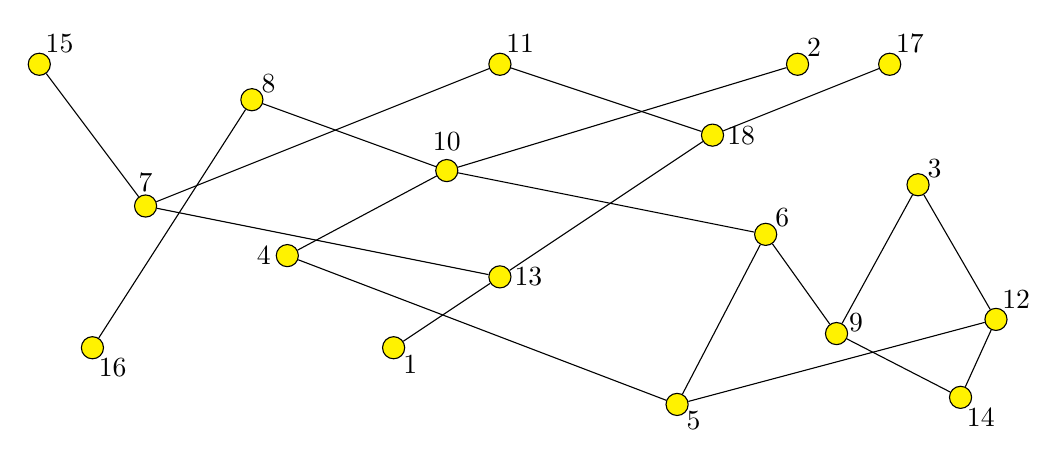
\begin{tikzpicture}
        [scale=0.9,every node/.style={draw,shape=circle,fill=yellow,inner sep=0,minimum size=8pt}, every draw/.style={line width=0.25mm, black}]

        \node[label=315:{1}] (v1) at (0, 0) {};
        \node[label=45:{2}] (v2) at (5.7, 4) {};
        \node[label=45:{3}] (v3) at (7.4, 2.3) {};
        \node[label=180:{4}] (v4) at (-1.5, 1.3) {};
        \node[label=315:{5}] (v5) at (4, -0.8) {};
        \node[label=45:{6}] (v6) at (5.25, 1.6) {};
        \node[label=90:{7}] (v7) at (-3.5, 2) {};
        \node[label=45:{8}] (v8) at (-2, 3.5) {};
        \node[label=15:{9}] (v9) at (6.25, 0.2) {};
        \node[label=90:{10}] (v10) at (0.75, 2.5) {};
        \node[label=45:{11}] (v11) at (1.5, 4) {};
        \node[label=45:{12}] (v12) at (8.5, 0.4) {};
        \node[label=0:{13}] (v13) at (1.5, 1) {};
        \node[label=315:{14}] (v14) at (8, -0.7) {};
        \node[label=45:{15}] (v15) at (-5, 4) {};
        \node[label=315:{16}] (v16) at (-4.25, 0) {};
        \node[label=45:{17}] (v17) at (7, 4) {};
        \node[label=0:{18}] (v18) at (4.5, 3) {};

        \draw (v1) -- (v13);
        \draw (v2) -- (v10);
        \draw (v3) -- (v9);
        \draw (v3) -- (v12);
        \draw (v4) -- (v5);
        \draw (v4) -- (v10);
        \draw (v5) -- (v6);
        \draw (v5) -- (v12);
        \draw (v6) -- (v9);
        \draw (v6) -- (v10);
        \draw (v7) -- (v11);
        \draw (v7) -- (v13);
        \draw (v7) -- (v15);
        \draw (v8) -- (v10);
        \draw (v8) -- (v16);
        \draw (v9) -- (v14);
        \draw (v11) -- (v18);
        \draw (v12) -- (v14);
        \draw (v13) -- (v18);
        \draw (v17) -- (v18);

      \end{tikzpicture}

    \end{figure}

    \begin{enumerate}[label={\alph*.}]
      \item List the maximal elements of \textbf{P}.
      \item List the minimal elements of \textbf{P}.
      \item Find a maximal chain with two points in \textbf{P}.
      \item Find a chain in \textbf{P} with three points that is \textit{not} maximal. Say why your chain is not maximal.
      \item Find a maximal antichain with four points in \textbf{P}.
    \end{enumerate}
  \end{problem}

  \begin{solution}
    \hfill
    \begin{enumerate}[label={\alph*.}]
      \item The maximal elements are 2, 3, 8, 11, 15, and 17.
      \item The minimal elements are 1, 5, 14, and 16.
      \item A maximal chain with two points is \(\{16, 8\}\).
      \item A chain with three points is \(\{5, 6, 10\}\). The chain is not maximal because the superset \(\{5, 6, 8, 10\}\) is also a chain.
      \item A maximal antichain with four points is \(\{1, 5, 14, 16\}\).
    \end{enumerate}
  \end{solution}

  % Problem 6.9
  \begin{problem}
    Find the height \(h\) of the poset \(\textbf{P} = \left(X, P\right)\) shown below as well as a maximum chain and a partition of \(X\) into \(h\) antichains using the algorithm from this chapter.

    \begin{figure}[H]
      \centering
      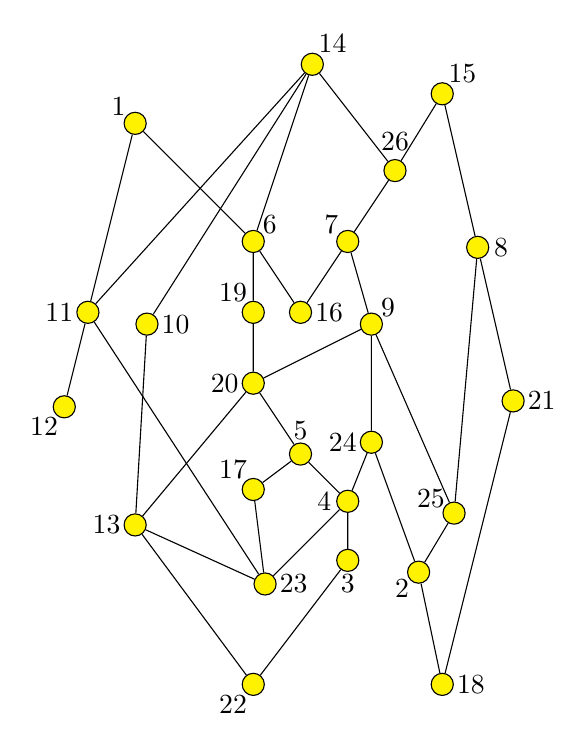
\begin{tikzpicture}
        [scale=1.5,every node/.style={draw,shape=circle,fill=yellow,inner sep=0,minimum size=8pt}, every draw/.style={line width=0.25mm, black}]

        \node[label=135:{1}] (v1) at (0, 0) {};
        \node[label=225:{2}] (v2) at (2.4, -3.8) {};
        \node[label=270:{3}] (v3) at (1.8, -3.7) {};
        \node[label=180:{4}] (v4) at (1.8, -3.2) {};
        \node[label=90:{5}] (v5) at (1.4, -2.8) {};
        \node[label=45:{6}] (v6) at (1, -1) {};
        \node[label=135:{7}] (v7) at (1.8, -1) {};
        \node[label=0:{8}] (v8) at (2.9, -1.05) {};
        \node[label=45:{9}] (v9) at (2, -1.7) {};
        \node[label=0:{10}] (v10) at (0.1, -1.7) {};
        \node[label=180:{11}] (v11) at (-0.4, -1.6) {};
        \node[label=225:{12}] (v12) at (-0.6, -2.4) {};
        \node[label=180:{13}] (v13) at (0, -3.4) {};
        \node[label=45:{14}] (v14) at (1.5, 0.5) {};
        \node[label=45:{15}] (v15) at (2.6, 0.25) {};
        \node[label=0:{16}] (v16) at (1.4, -1.6) {};
        \node[label=135:{17}] (v17) at (1, -3.1) {};
        \node[label=0:{18}] (v18) at (2.6, -4.75) {};
        \node[label=135:{19}] (v19) at (1, -1.6) {};
        \node[label=180:{20}] (v20) at (1, -2.2) {};
        \node[label=0:{21}] (v21) at (3.2, -2.35) {};
        \node[label=225:{22}] (v22) at (1, -4.75) {};
        \node[label=0:{23}] (v23) at (1.1, -3.9) {};
        \node[label=180:{24}] (v24) at (2, -2.7) {};
        \node[label=165:{25}] (v25) at (2.7, -3.3) {};
        \node[label=90:{26}] (v26) at (2.2, -0.4) {};

        \draw (v1) -- (v6);
        \draw (v1) -- (v11);
        \draw (v2) -- (v18);
        \draw (v2) -- (v24);
        \draw (v2) -- (v25);
        \draw (v3) -- (v4);
        \draw (v3) -- (v22);
        \draw (v4) -- (v5);
        \draw (v4) -- (v23);
        \draw (v4) -- (v24);
        \draw (v5) -- (v17);
        \draw (v5) -- (v20);
        \draw (v6) -- (v14);
        \draw (v6) -- (v16);
        \draw (v6) -- (v19);
        \draw (v7) -- (v9);
        \draw (v7) -- (v16);
        \draw (v7) -- (v26);
        \draw (v8) -- (v15);
        \draw (v8) -- (v21);
        \draw (v8) -- (v25);
        \draw (v9) -- (v20);
        \draw (v9) -- (v24);
        \draw (v9) -- (v25);
        \draw (v10) -- (v13);
        \draw (v10) -- (v14);
        \draw (v11) -- (v12);
        \draw (v11) -- (v14);
        \draw (v11) -- (v23);
        \draw (v13) -- (v20);
        \draw (v13) -- (v22);
        \draw (v13) -- (v23);
        \draw (v14) -- (v26);
        \draw (v15) -- (v26);
        \draw (v17) -- (v23);
        \draw (v18) -- (v21);
        \draw (v19) -- (v20);
      \end{tikzpicture}

    \end{figure}
  \end{problem}

  \begin{solution}
    The height of the poset \textbf{P} is 9 and a maximum chain is \{22, 3, 4, 5, 20, 9, 7, 26, 15\}. The poset can be partitioned into the following antichains:
    \begin{align*}
      A_{1} &= \{12, 16, 18, 22, 23\} \\
      A_{2} &= \{2, 3, 11, 13, 17, 21\} \\
      A_{3} &= \{4, 10, 25\} \\
      A_{4} &= \{5, 8, 24\} \\
      A_{5} &= \{20\} \\
      A_{6} &= \{9, 19\} \\
      A_{7} &= \{6, 7\} \\
      A_{8} &= \{1, 26\} \\
      A_{9} &= \{14, 15\}
    \end{align*}
  \end{solution}

  % Problem 6.11
  \setcounter{problem-internal}{10}
  \begin{problem}
    A restaurant chef has designed a new set of dishes for his menu. His set of dishes contains 10 main courses, and he will select a subset of them to place on the menu each night. To ensure variety of main courses for his patrons, he wants to guarantee that a night's menu is neither completely contained in nor completely contains another night's menu. What is the largest number of menus he can plan using his 10 main courses subject to this requirement?
  \end{problem}

  \begin{solution}
    Let \(\textbf{P}_{n}\) denote the poset defined by the power set on \(n\) elements with ordering by inclusion. Note that each element of \(\textbf{P}_{n}\) is a collection of dishes, or a menu, and our chef wants to guarantee that no two menus are subsets of one another. That is, no two elements should be comparable. Recall that a set in which no two elements are comparable is an antichain. Then our problem is equivalent to finding the maximum size of an antichain, or the width \(w\) of \(\textbf{P}_{n}\).

    Notice that the order diagram for \(\textbf{P}_{n}\) can be represented as \(n\) rows, where the \(i\)-th row contains the subsets with order \(i\). Thus, the \(i\)-th row has \({n \choose i}\) elements of \(\textbf{P}_{n}\). Furthermore, a subset \(A\) of order \(i\) is covered by exactly \(n - i\) subsets (namely the sets containing the elements of \(A\) and one of the remaining \(n - i\) elements).

    We first show that \(\textbf{P}_{n}\) can be partitioned into \(C\left(n, \lfloor{\frac{n}{2}}\rfloor\right)\) chains. We do so by induction. For the base case, let \(n = 1\). Then the powerset of \(S\) has two elements, namely \(\emptyset\) and \(\{1\}\). Clearly \(\emptyset \subseteq \{1\}\) so we can form a chain with these two elements and we are done, since \(1 = C\left(1, 0\right)\). Now suppose the statement holds for \(n = k\) where \(k \geq 1\). Let \(n = k+1\) and we will treat two separate cases.

    Suppose first that \(k + 1\) is even. Ignore all subsets of \(S\) that contain the element \(k + 1\), of which there are \(2^{k}\). The remaining subsets are the powerset on \(k\) elements. By the induction hypothesis, we can partition this into \(C\left(k, \lfloor{\frac{k}{2}}\rfloor\right)\) chains. The remaining subsets all contain \(k+1\) and some collection of the remaining \(k\) elements to choose from. As a result, they can be interpreted as the powerset on \(k\) elements and can also be partitioned into \(C\left(k, \lfloor{\frac{k}{2}}\rfloor\right)\) chains. In total, we've partitioned our poset into \(2 \cdot C\left(k, \lfloor{\frac{k}{2}}\rfloor\right)\) chains. Note that since \(k+1\) is even and \(k\) is odd, we have \(\lfloor{\frac{k+1}{2}}\rfloor = \frac{k+1}{2}\) and \(\lfloor{\frac{k}{2}}\rfloor = \frac{k - 1}{2} = \frac{k + 1}{2} - 1\). Then we have the following
    \begin{align*}
      2 \cdot {k \choose \frac{k+1}{2} - 1} &= 2 \cdot \frac{k!}{\left(\frac{k+1}{2}\right)! \left(\frac{k+1}{2} - 1\right)!} \\
      &= 2 \cdot \frac{\frac{k+1}{2}}{\frac{k+1}{2}} \cdot \frac{k!}{\left(\frac{k+1}{2}\right)! \left(\frac{k+1}{2} - 1\right)!} \\
      &= \frac{\left(k+1\right) k!}{\left(\frac{k+1}{2}\right)! \left(\frac{k+1}{2}\right) \left(\frac{k+1}{2} - 1\right)!} \\
      &= \frac{\left(k + 1\right)!}{\left(\frac{k+1}{2}\right)! \left(\frac{k+1}{2}\right)!} \\
      &= {k+1 \choose \lfloor{\frac{k + 1}{2}}\rfloor}
    \end{align*}
    Thus, the statement holds when \(k + 1\) is even.

    Now suppose \(k + 1\) is odd. We form a partition on of \(\textbf{P}_{k+1}\) by extending the chains which partition \(\textbf{P}_{k}\). Suppose the chain \(C_{i}\) has maximal element \(A_{i, m}\) in \(\textbf{P}_{k}\). Then the new maximal element of \(C_{i}\) in \(\textbf{P}_{k+1}\) is \(A_{i, m} \cup \{k+1\}\). For example, the chain \(\emptyset \subset \{1\} \subset \{1, 2\}\) has \(\{1, 2, 3\}\) appended to the end when going from \(\textbf{P}_{2}\) to \(\textbf{P}_{3}\). Furthermore, for every \(C_{i}\), consider the new chain in which every set of \(C_{i}\) is unioned with \(\{k+1\}\). The maximal element of these new chains \(C'_{i}\) should be one set below those of the chains in the first step. Reusing the example from before, our new chain would be \(\{3\} \subset \{1, 3\}\). Our first step guarantees every element of \(\textbf{P}_{k}\) is in a chain. The extension and the second step ensures every element of \(\textbf{P}_{k+1}\) which contains \(k+1\) is in a chain. Therefore, every element of \(\textbf{P}_{k+1}\) is in a unique chain so this is a partition.

    First note that since \(k+1\) is odd and \(k\) is even, we have \(\lfloor{\frac{k+1}{2}}\rfloor = \lfloor{\frac{k}{2}}\rfloor = \frac{k}{2}\). In the first step of the above process, we formed \(C\left(k, \lfloor{\frac{k}{2}}\rfloor\right)\) chains by extension, one for each chain in the partition of \(\textbf{P}_{k}\). The second step involves creating a new chain for each subset of order \(\lfloor{\frac{k}{2}}\rfloor\) containing the element \(k+1\). There are precisely \(C\left(k+1, \frac{k}{2}\right) - C\left(k, \frac{k}{2}\right)\) of these subsets (each chain formed by this step either starts at subsets of this size or starts earlier but contains exactly one subset of this size). Summing the two numbers of chains formed, we find that there are a total of \(C\left(k+1, \lfloor{\frac{k+1}{2}}\rfloor\right)\) chains in our partition of \(\textbf{P}_{k+1}\). Thus, the statement holds when \(k+1\) is odd.
    % Let \(A\) be a subset of the specified size. If \(k+1 \notin A\), then \(A\) is part of a unique chain extension. If \(k+1 \in A\), then \(A\) is either the maximal element of an extension, or \(A\) is in one of our constructed chains (including the ones of trivial length). Since each set of size \(\lfloor{\frac{n}{2}}\rfloor\) belongs to exactly one chain, and there are \(C\left(n, \lfloor{\frac{n}{2}}\rfloor\right)\) such sets, there must be \(C\left(n, \lfloor{\frac{n}{2}}\rfloor\right)\) chains. Thus the statement holds for \(k+1\) odd.

    We have proven that \(\textbf{P}_{n}\) can be partitioned into \(C\left(n, \lfloor{\frac{n}{2}}\rfloor\right)\) chains. By Dilworth's Theorem, this value is an upper bound on the width of \(\textbf{P}_{n}\).

    Now we show that there is an antichain of size \(C\left(n, \lfloor{\frac{n}{2}}\rfloor\right)\). Let \(A\) be the collection of elements in \(\textbf{P}_{n}\) of size \(\lfloor{\frac{n}{2}}\rfloor\). The size of \(A\) is equal to the number of subsets of \(S\) of size \(\lfloor{\frac{n}{2}}\rfloor\), which is \(C\left(n, \lfloor{\frac{n}{2}}\rfloor\right)\). Since each set in \(A\) is equal in size but distinct, no two sets can contain one another and no two sets are comparable. Thus, \(A\) is an antichain of size \(C\left(n, \lfloor{\frac{n}{2}}\rfloor\right)\). Since this is equal to the upper bound shown earlier, the antichain is of maximum size and we have proven that the width of \(\textbf{P}_{n}\) is \(C\left(n, \lfloor{\frac{n}{2}}\rfloor\right)\).

    In the particular case for our problem where \(n = 10\), the largest number of menus the chef can plan is \({10 \choose 5} = 252\).

    % Now we show that \(\textbf{P}_{n}\) can be partitioned into \(C\left(n, \lfloor{\frac{n}{2}}\rfloor\right)\) chains. We do so by induction. For the base case, let \(n = 1\). Then the powerset of \(S\) has two elements, namely \(\emptyset\) and \(\{1\}\). Clearly \(\emptyset \subseteq \{1\}\) so we can form a chain with these two elements and we are done, since \(1 = C\left(1, 0\right)\). Now suppose the statement holds for \(n = k\) where \(k \geq 1\). Let \(n = k+1\) and we will partition this poset into chains.
    %
    % Start by extending the chains in the partition of \(\textbf{P}_{k}\). Suppose the chain \(C_{i}\) has maximal element \(A_{i, m}\) in \(\textbf{P}_{k}\). Then the new maximal element of \(C_{i}\) in \(\textbf{P}_{k+1}\) is \(A_{i, m} \cup \{k+1\}\).

    % In general, the width of the powerset on \(n\) elements ordered by inclusion is \(C\left(n, \lfloor{\frac{n}{2}}\rfloor\right)\)

  \end{solution}

\end{document}
